%%%%%%%%%%%%%%%%%%%%%%%%%%%%%%%%%%%%%%%%%
% The Legrand Orange Book
% LaTeX Template
% Version 1.4 (12/4/14)
%
% This template has been downloaded from:
% http://www.LaTeXTemplates.com
%
% Original author:
% Mathias Legrand (legrand.mathias@gmail.com)
%
% License:
% CC BY-NC-SA 3.0 (http://creativecommons.org/licenses/by-nc-sa/3.0/)
%
% Compiling this template:
% This template uses biber for its bibliography and makeindex for its index.
% When you first open the template, compile it from the command line with the
% commands below to make sure your LaTeX distribution is configured correctly:
%
% 1) pdflatex main
% 2) makeindex main.idx -s StyleInd.ist
% 3) biber main
% 4) pdflatex main x 2
%
% After this, when you wish to update the bibliography/index use the appropriate
% command above and make sure to compile with pdflatex several times
% afterwards to propagate your changes to the document.
%
% This template also uses a number of packages which may need to be
% updated to the newest versions for the template to compile. It is strongly
% recommended you update your LaTeX distribution if you have any
% compilation errors.
%
% Important note:
% Chapter heading images should have a 2:1 width:height ratio,
% e.g. 920px width and 460px height.
%
%%%%%%%%%%%%%%%%%%%%%%%%%%%%%%%%%%%%%%%%%

%----------------------------------------------------------------------------------------
%	PACKAGES AND OTHER DOCUMENT CONFIGURATIONS
%----------------------------------------------------------------------------------------

\documentclass[11pt,fleqn]{book} % Default font size and left-justified equations

\usepackage[top=3cm,bottom=3cm,left=3.2cm,right=3.2cm,headsep=10pt,a4paper]{geometry} % Page margins
\usepackage{placeins}
\usepackage{xcolor} % Required for specifying colors by name
\definecolor{ocre}{RGB}{243,102,25} % Define the orange color used for highlighting throughout the book

% Font Settings
\usepackage{avant} % Use the Avantgarde font for headings
%\usepackage{times} % Use the Times font for headings
\usepackage{mathptmx} % Use the Adobe Times Roman as the default text font together with math symbols from the Sym­bol, Chancery and Com­puter Modern fonts

\usepackage{microtype} % Slightly tweak font spacing for aesthetics
\usepackage[utf8]{inputenc} % Required for including letters with accents
\usepackage[T1]{fontenc} % Use 8-bit encoding that has 256 glyphs

%haestrod
\usepackage{amssymb}
\usepackage{xfrac}
\usepackage{multicol}
\setlength{\columnsep}{-15 pt}
\usepackage{wrapfig}
\usepackage{mathtools}
\usepackage{amsfonts}
\usepackage{tcolorbox}

% Resizing tables
\usepackage{tabulary}

% Bibliography
\usepackage[style=alphabetic,sorting=nyt,sortcites=true,autopunct=true,babel=hyphen,hyperref=true,abbreviate=false,backref=true,backend=biber]{biblatex}
\addbibresource{bibliography.bib} % BibTeX bibliography file
\defbibheading{bibempty}{}

% Index
\usepackage{calc} % For simpler calculation - used for spacing the index letter headings correctly
\usepackage{makeidx} % Required to make an index
\makeindex % Tells LaTeX to create the files required for indexing

%----------------------------------------------------------------------------------------

%----------------------------------------------------------------------------------------
%	VARIOUS REQUIRED PACKAGES
%----------------------------------------------------------------------------------------

\usepackage{titlesec} % Allows customization of titles

\usepackage{graphicx} % Required for including pictures
\graphicspath{{Pictures/}} % Specifies the directory where pictures are stored

\usepackage{lipsum} % Inserts dummy text

\usepackage{tikz} % Required for drawing custom shapes

\usepackage[english]{babel} % English language/hyphenation

\usepackage{enumitem} % Customize lists
\setlist{nolistsep} % Reduce spacing between bullet points and numbered lists

\usepackage{booktabs} % Required for nicer horizontal rules in tables

\usepackage{eso-pic} % Required for specifying an image background in the title page

%----------------------------------------------------------------------------------------
%	MAIN TABLE OF CONTENTS
%----------------------------------------------------------------------------------------

\usepackage{titletoc} % Required for manipulating the table of contents

\contentsmargin{0cm} % Removes the default margin
% Chapter text styling
\titlecontents{chapter}[1.25cm] % Indentation
{\addvspace{15pt}\large\sffamily\bfseries} % Spacing and font options for chapters
{\color{ocre!60}\contentslabel[\Large\thecontentslabel]{1.25cm}\color{ocre}} % Chapter number
{}  
{\color{ocre!60}\normalsize\sffamily\bfseries\;\titlerule*[.5pc]{.}\;\thecontentspage} % Page number
% Section text styling
\titlecontents{section}[1.25cm] % Indentation
{\addvspace{5pt}\sffamily\bfseries} % Spacing and font options for sections
{\contentslabel[\thecontentslabel]{1.25cm}} % Section number
{}
{\sffamily\hfill\color{black}\thecontentspage} % Page number
[]
% Subsection text styling
\titlecontents{subsection}[1.25cm] % Indentation
{\addvspace{1pt}\sffamily\small} % Spacing and font options for subsections
{\contentslabel[\thecontentslabel]{1.25cm}} % Subsection number
{}
{\sffamily\;\titlerule*[.5pc]{.}\;\thecontentspage} % Page number
[] 

%----------------------------------------------------------------------------------------
%	MINI TABLE OF CONTENTS IN CHAPTER HEADS
%----------------------------------------------------------------------------------------

% Section text styling
\titlecontents{lsection}[0em] % Indendating
{\footnotesize\sffamily} % Font settings
{}
{}
{}

% Subsection text styling
\titlecontents{lsubsection}[.5em] % Indentation
{\normalfont\footnotesize\sffamily} % Font settings
{}
{}
{}
 
%----------------------------------------------------------------------------------------
%	PAGE HEADERS
%----------------------------------------------------------------------------------------

\usepackage{fancyhdr} % Required for header and footer configuration

\pagestyle{fancy}
\renewcommand{\chaptermark}[1]{\markboth{\sffamily\normalsize\bfseries\chaptername\ \thechapter.\ #1}{}} % Chapter text font settings
\renewcommand{\sectionmark}[1]{\markright{\sffamily\normalsize\thesection\hspace{5pt}#1}{}} % Section text font settings
\fancyhf{} \fancyhead[LE,RO]{\sffamily\normalsize\thepage} % Font setting for the page number in the header
\fancyhead[LO]{\rightmark} % Print the nearest section name on the left side of odd pages
\fancyhead[RE]{\leftmark} % Print the current chapter name on the right side of even pages
\renewcommand{\headrulewidth}{0.5pt} % Width of the rule under the header
\addtolength{\headheight}{2.5pt} % Increase the spacing around the header slightly
\renewcommand{\footrulewidth}{0pt} % Removes the rule in the footer
\fancypagestyle{plain}{\fancyhead{}\renewcommand{\headrulewidth}{0pt}} % Style for when a plain pagestyle is specified

% Removes the header from odd empty pages at the end of chapters
\makeatletter
\renewcommand{\cleardoublepage}{
\clearpage\ifodd\c@page\else
\hbox{}
\vspace*{\fill}
\thispagestyle{empty}
\newpage
\fi}

%----------------------------------------------------------------------------------------
%	THEOREM STYLES
%----------------------------------------------------------------------------------------

\usepackage{amsmath,amsfonts,amssymb,amsthm} % For math equations, theorems, symbols, etc

\newcommand{\intoo}[2]{\mathopen{]}#1\,;#2\mathclose{[}}
\newcommand{\ud}{\mathop{\mathrm{{}d}}\mathopen{}}
\newcommand{\intff}[2]{\mathopen{[}#1\,;#2\mathclose{]}}
\newtheorem{notation}{Notation}[chapter]

%%%%%%%%%%%%%%%%%%%%%%%%%%%%%%%%%%%%%%%%%%%%%%%%%%%%%%%%%%%%%%%%%%%%%%%%%%%
%%%%%%%%%%%%%%%%%%%% dedicated to boxed/framed environements %%%%%%%%%%%%%%
%%%%%%%%%%%%%%%%%%%%%%%%%%%%%%%%%%%%%%%%%%%%%%%%%%%%%%%%%%%%%%%%%%%%%%%%%%%
\newtheoremstyle{ocrenumbox}% % Theorem style name
{0pt}% Space above
{0pt}% Space below
{\normalfont}% % Body font
{}% Indent amount
{\small\bf\sffamily\color{ocre}}% % Theorem head font
{\;}% Punctuation after theorem head
{0.25em}% Space after theorem head
{\small\sffamily\color{ocre}\thmname{#1}\nobreakspace\thmnumber{\@ifnotempty{#1}{}\@upn{#2}}% Theorem text (e.g. Theorem 2.1)
\thmnote{\nobreakspace\the\thm@notefont\sffamily\bfseries\color{black}---\nobreakspace#3.}} % Optional theorem note
\renewcommand{\qedsymbol}{$\blacksquare$}% Optional qed square

\newtheoremstyle{blacknumex}% Theorem style name
{5pt}% Space above
{5pt}% Space below
{\normalfont}% Body font
{} % Indent amount
{\small\bf\sffamily}% Theorem head font
{\;}% Punctuation after theorem head
{0.25em}% Space after theorem head
{\small\sffamily{\tiny\ensuremath{\blacksquare}}\nobreakspace\thmname{#1}\nobreakspace\thmnumber{\@ifnotempty{#1}{}\@upn{#2}}% Theorem text (e.g. Theorem 2.1)
\thmnote{\nobreakspace\the\thm@notefont\sffamily\bfseries---\nobreakspace#3.}}% Optional theorem note

\newtheoremstyle{blacknumbox} % Theorem style name
{0pt}% Space above
{0pt}% Space below
{\normalfont}% Body font
{}% Indent amount
{\small\bf\sffamily}% Theorem head font
{\;}% Punctuation after theorem head
{0.25em}% Space after theorem head
{\small\sffamily\thmname{#1}\nobreakspace\thmnumber{\@ifnotempty{#1}{}\@upn{#2}}% Theorem text (e.g. Theorem 2.1)
\thmnote{\nobreakspace\the\thm@notefont\sffamily\bfseries---\nobreakspace#3.}}% Optional theorem note

%%%%%%%%%%%%%%%%%%%%%%%%%%%%%%%%%%%%%%%%%%%%%%%%%%%%%%%%%%%%%%%%%%%%%%%%%%%
%%%%%%%%%%%%% dedicated to non-boxed/non-framed environements %%%%%%%%%%%%%
%%%%%%%%%%%%%%%%%%%%%%%%%%%%%%%%%%%%%%%%%%%%%%%%%%%%%%%%%%%%%%%%%%%%%%%%%%%
\newtheoremstyle{ocrenum}% % Theorem style name
{5pt}% Space above
{5pt}% Space below
{\normalfont}% % Body font
{}% Indent amount
{\small\bf\sffamily\color{ocre}}% % Theorem head font
{\;}% Punctuation after theorem head
{0.25em}% Space after theorem head
{\small\sffamily\color{ocre}\thmname{#1}\nobreakspace\thmnumber{\@ifnotempty{#1}{}\@upn{#2}}% Theorem text (e.g. Theorem 2.1)
\thmnote{\nobreakspace\the\thm@notefont\sffamily\bfseries\color{black}---\nobreakspace#3.}} % Optional theorem note
\renewcommand{\qedsymbol}{$\blacksquare$}% Optional qed square
\makeatother

% Defines the theorem text style for each type of theorem to one of the three styles above
\newcounter{dummy} 
\numberwithin{dummy}{section}
\theoremstyle{ocrenumbox}
\newtheorem{theoremeT}[dummy]{Theorem}
\newtheorem{problem}{Problem}[chapter]
\newtheorem{exerciseT}{Exercise}[chapter]
\theoremstyle{blacknumex}
\newtheorem{exampleT}{Example}[chapter]
\theoremstyle{blacknumbox}
\newtheorem{vocabulary}{Vocabulary}[chapter]
\newtheorem{definitionT}{Definition}[section]
\newtheorem{corollaryT}[dummy]{Corollary}
\theoremstyle{ocrenum}
\newtheorem{proposition}[dummy]{Proposition}

%----------------------------------------------------------------------------------------
%	DEFINITION OF COLORED BOXES
%----------------------------------------------------------------------------------------

\RequirePackage[framemethod=default]{mdframed} % Required for creating the theorem, definition, exercise and corollary boxes

% Theorem box
\newmdenv[skipabove=7pt,
skipbelow=7pt,
backgroundcolor=black!5,
linecolor=ocre,
innerleftmargin=5pt,
innerrightmargin=5pt,
innertopmargin=5pt,
leftmargin=0cm,
rightmargin=0cm,
innerbottommargin=5pt]{tBox}

% Exercise box	  
\newmdenv[skipabove=7pt,
skipbelow=7pt,
rightline=false,
leftline=true,
topline=false,
bottomline=false,
backgroundcolor=ocre!10,
linecolor=ocre,
innerleftmargin=5pt,
innerrightmargin=5pt,
innertopmargin=5pt,
innerbottommargin=5pt,
leftmargin=0cm,
rightmargin=0cm,
linewidth=4pt]{eBox}	

% Definition box
\newmdenv[skipabove=7pt,
skipbelow=7pt,
rightline=false,
leftline=true,
topline=false,
bottomline=false,
linecolor=ocre,
innerleftmargin=5pt,
innerrightmargin=5pt,
innertopmargin=0pt,
leftmargin=0cm,
rightmargin=0cm,
linewidth=4pt,
innerbottommargin=0pt]{dBox}	

% Corollary box
\newmdenv[skipabove=7pt,
skipbelow=7pt,
rightline=false,
leftline=true,
topline=false,
bottomline=false,
linecolor=gray,
backgroundcolor=black!5,
innerleftmargin=5pt,
innerrightmargin=5pt,
innertopmargin=5pt,
leftmargin=0cm,
rightmargin=0cm,
linewidth=4pt,
innerbottommargin=5pt]{cBox}

% Creates an environment for each type of theorem and assigns it a theorem text style from the "Theorem Styles" section above and a colored box from above
\newenvironment{theorem}{\begin{tBox}\begin{theoremeT}}{\end{theoremeT}\end{tBox}}
\newenvironment{exercise}{\begin{eBox}\begin{exerciseT}}{\hfill{\color{ocre}\tiny\ensuremath{\blacksquare}}\end{exerciseT}\end{eBox}}				  
\newenvironment{definition}{\begin{dBox}\begin{definitionT}}{\end{definitionT}\end{dBox}}	
\newenvironment{example}{\begin{exampleT}}{\hfill{\tiny\ensuremath{\blacksquare}}\end{exampleT}}		
\newenvironment{corollary}{\begin{cBox}\begin{corollaryT}}{\end{corollaryT}\end{cBox}}	

%----------------------------------------------------------------------------------------
%	REMARK ENVIRONMENT
%----------------------------------------------------------------------------------------

\newenvironment{remark}{\par\vspace{10pt}\small % Vertical white space above the remark and smaller font size
\begin{list}{}{
\leftmargin=35pt % Indentation on the left
\rightmargin=25pt}\item\ignorespaces % Indentation on the right
\makebox[-2.5pt]{\begin{tikzpicture}[overlay]
\node[draw=ocre!60,line width=1pt,circle,fill=ocre!25,font=\sffamily\bfseries,inner sep=2pt,outer sep=0pt] at (-15pt,0pt){\textcolor{ocre}{R}};\end{tikzpicture}} % Orange R in a circle
\advance\baselineskip -1pt}{\end{list}\vskip5pt} % Tighter line spacing and white space after remark

%----------------------------------------------------------------------------------------
%	SECTION NUMBERING IN THE MARGIN
%----------------------------------------------------------------------------------------

\makeatletter
\renewcommand{\@seccntformat}[1]{\llap{\textcolor{ocre}{\csname the#1\endcsname}\hspace{1em}}}                    
\renewcommand{\section}{\@startsection{section}{1}{\z@}
{-4ex \@plus -1ex \@minus -.4ex}
{1ex \@plus.2ex }
{\normalfont\large\sffamily\bfseries}}
\renewcommand{\subsection}{\@startsection {subsection}{2}{\z@}
{-3ex \@plus -0.1ex \@minus -.4ex}
{0.5ex \@plus.2ex }
{\normalfont\sffamily\bfseries}}
\renewcommand{\subsubsection}{\@startsection {subsubsection}{3}{\z@}
{-2ex \@plus -0.1ex \@minus -.2ex}
{.2ex \@plus.2ex }
{\normalfont\small\sffamily\bfseries}}                        
\renewcommand\paragraph{\@startsection{paragraph}{4}{\z@}
{-2ex \@plus-.2ex \@minus .2ex}
{.1ex}
{\normalfont\small\sffamily\bfseries}}

%----------------------------------------------------------------------------------------
%	HYPERLINKS IN THE DOCUMENTS
%----------------------------------------------------------------------------------------

% For an unclear reason, the package should be loaded now and not later
\usepackage{hyperref}
\hypersetup{hidelinks,backref=true,pagebackref=true,hyperindex=true,colorlinks=false,breaklinks=true,urlcolor= ocre,bookmarks=true,bookmarksopen=false,pdftitle={Title},pdfauthor={Author}}

%----------------------------------------------------------------------------------------
%	CHAPTER HEADINGS
%----------------------------------------------------------------------------------------

% The set-up below should be (sadly) manually adapted to the overall margin page septup controlled by the geometry package loaded in the main.tex document. It is possible to implement below the dimensions used in the goemetry package (top,bottom,left,right)... TO BE DONE

\newcommand{\thechapterimage}{}
\newcommand{\chapterimage}[1]{\renewcommand{\thechapterimage}{#1}}

% Numbered chapters with mini tableofcontents
\def\thechapter{\arabic{chapter}}
\def\@makechapterhead#1{
\thispagestyle{empty}
{\centering \normalfont\sffamily
\ifnum \c@secnumdepth >\m@ne
\if@mainmatter
\startcontents
\begin{tikzpicture}[remember picture,overlay]
\node at (current page.north west)
{\begin{tikzpicture}[remember picture,overlay]
\node[anchor=north west,inner sep=0pt] at (0,0) {\includegraphics[width=\paperwidth]{\thechapterimage}};
%%%%%%%%%%%%%%%%%%%%%%%%%%%%%%%%%%%%%%%%%%%%%%%%%%%%%%%%%%%%%%%%%%%%%%%%%%%%%%%%%%%%%
% Commenting the 3 lines below removes the small contents box in the chapter heading
\fill[color=ocre!10!white,opacity=.6] (1cm,0) rectangle (8cm,-7cm);
\node[anchor=north west] at (1.1cm,.35cm) {\parbox[t][8cm][t]{6.5cm}{\huge\bfseries\flushleft \printcontents{l}{1}{\setcounter{tocdepth}{2}}}};
\draw[anchor=west] (5cm,-9cm) node [rounded corners=20pt,fill=ocre!10!white,text opacity=1,draw=ocre,draw opacity=1,line width=1.5pt,fill opacity=.6,inner sep=12pt]{\huge\sffamily\bfseries\textcolor{black}{\thechapter. #1\strut\makebox[22cm]{}}};
%%%%%%%%%%%%%%%%%%%%%%%%%%%%%%%%%%%%%%%%%%%%%%%%%%%%%%%%%%%%%%%%%%%%%%%%%%%%%%%%%%%%%
\end{tikzpicture}};
\end{tikzpicture}}
\par\vspace*{230\p@}
\fi
\fi}

% Unnumbered chapters without mini tableofcontents (could be added though) 
\def\@makeschapterhead#1{
\thispagestyle{empty}
{\centering \normalfont\sffamily
\ifnum \c@secnumdepth >\m@ne
\if@mainmatter
\begin{tikzpicture}[remember picture,overlay]
\node at (current page.north west)
{\begin{tikzpicture}[remember picture,overlay]
\node[anchor=north west,inner sep=0pt] at (0,0) {\includegraphics[width=\paperwidth]{\thechapterimage}};
\draw[anchor=west] (5cm,-9cm) node [rounded corners=20pt,fill=ocre!10!white,fill opacity=.6,inner sep=12pt,text opacity=1,draw=ocre,draw opacity=1,line width=1.5pt]{\huge\sffamily\bfseries\textcolor{black}{#1\strut\makebox[22cm]{}}};
\end{tikzpicture}};
\end{tikzpicture}}
\par\vspace*{230\p@}
\fi
\fi
}
\makeatother % Insert the commands.tex file which contains the majority of the structure behind the template

\begin{document}

%----------------------------------------------------------------------------------------
%	TITLE PAGE
%----------------------------------------------------------------------------------------

\begingroup
\thispagestyle{empty}
\AddToShipoutPicture*{\put(6,5){
\includegraphics[scale=1]{background}}} % Image background
\centering
\vspace*{9cm}
\par\normalfont\fontsize{35}{35}\sffamily\selectfont
Analog Integrated Circuit Design\par % Book title
\normalfont\fontsize{30}{30}\sffamily\selectfont
ECE 5021\par
\vspace*{1cm}
{\Huge Hardolaf \& Haestrod}\par % Author name
\endgroup

%----------------------------------------------------------------------------------------
%	COPYRIGHT PAGE
%----------------------------------------------------------------------------------------

\newpage
~\vfill
\thispagestyle{empty}

\noindent Copyright \copyright\ 2015 Hardolaf \& Haestrod\\ % Copyright notice

\noindent \textsc{Published by The Internet}\\ % Publisher

\noindent \textsc{hmpg.net}\\ % URL

\noindent Licensed under the Creative Commons Attribution-NonCommercial 3.0 Unported License (the ``License''). You may not use this file except in compliance with the License. You may obtain a copy of the License at \url{http://creativecommons.org/licenses/by-nc/3.0}. Unless required by applicable law or agreed to in writing, software distributed under the License is distributed on an \textsc{``as is'' basis, without warranties or conditions of any kind}, either express or implied. See the License for the specific language governing permissions and limitations under the License.\\ % License information

\noindent \textit{First printing, Never} % Printing/edition date

%----------------------------------------------------------------------------------------
%	TABLE OF CONTENTS
%----------------------------------------------------------------------------------------

\chapterimage{chapter_head_1.pdf} % Table of contents heading image

\pagestyle{empty} % No headers

\tableofcontents % Print the table of contents itself

\cleardoublepage % Forces the first chapter to start on an odd page so it's on the right

\pagestyle{fancy} % Print headers again

%----------------------------------------------------------------------------------------
%	CHAPTER 1
%----------------------------------------------------------------------------------------

\chapterimage{chapter_head_2.pdf} % Chapter heading image

\chapter{Introduction to Analog Signal Processing}

\section{Signals and Systems}\index{Signals and Systems}

\begin{figure}[h]
  \centering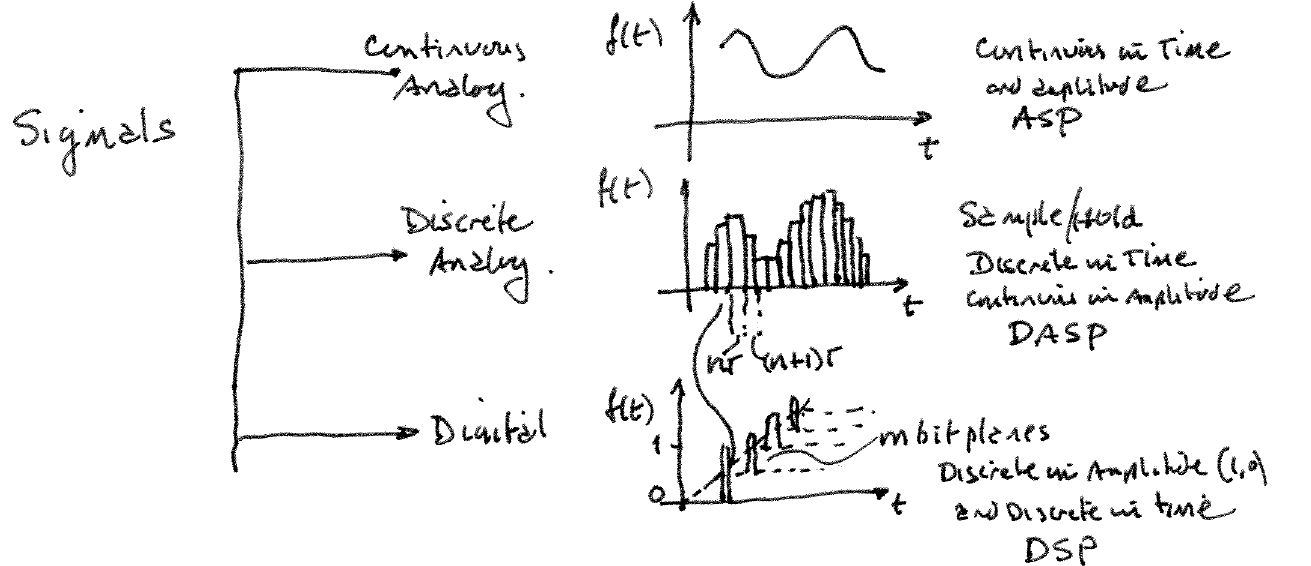
\includegraphics[scale=0.5]{chapter1_signals_and_systems.png}
  \caption{The three ways of representing signals in  time.}
\end{figure}

% -----------------------------------------------

\section{Signals}\index{Signals}

\begin{table}[h]
  \centering
  \begin{tabular}{l|l|l}
    \textbf{Analog (ASP)} & \textbf{Digital (DSP)} & \textbf{Discrete Analog (ASP)}\\
    Continuous in time & Discrete in time & Discrete in time \\
    Continuous in amplitude & Discrete in amplitude & Continuous in amplitude \\
    Differential equations & Difference equations & Difference equations \\
    Convolution integral & Discrete convolution & Discrete convolution \\
    Impulse response & Unit sampler & Unit sampler \\
    Laplace Transform & z-transform & Laplace and z-transforms \\
    s-plane & z-plane & s and z-planes\\
  \end{tabular}
  \caption{Comparison of the properties of the three types of signals.}
\end{table}

Discrete Analog Signal Processing (DASP) is a hybrid method of processing analog signals (continuously varying)

%------------------------------------------------

\section{Analog versus Digital}

\subsection{Considerations}\index{Analog versus Digital!Considerations}

\begin{table}[h]
  \centering
  \begin{tabulary}{1\textwidth}{lll}
    $\bullet$ Architechture/Algorithms & $\bullet$ S/N ratios & $\bullet$ Size \\
    $\bullet$ I/O requirements & $\bullet$ Dynamic range & $\bullet$ Weight \\
    $\bullet$ Bandwidth (TBWP) & $\bullet$ Linearity & $\bullet$ Cost \\
    $\bullet$ Precision & $\bullet$ Distortion &  \\
    $\bullet$ Sensor-based Systems & $\bullet$ Stability & \\
    $\bullet$ Programmability & $\bullet$ Power Dissipation &  \\
  \end{tabulary}
\end{table}

\begin{figure}[h]
  \centering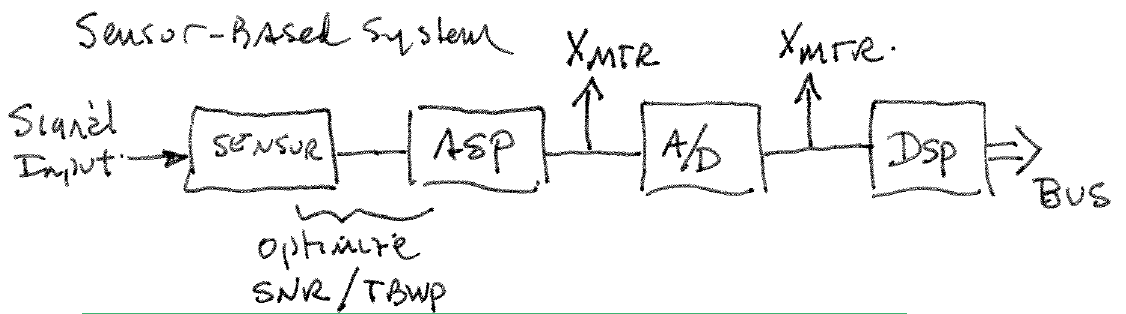
\includegraphics[scale=0.5]{chapter1_sensor-based-systems.png}
  \caption{Sensor-based System}
\end{figure}

%------------------------------------------------

\subsection{Scaled CMOS}\index{Analog versus Digital!Scaled CMOS}

\begin{description}
 \item General Rules \\
  \emph Analog is the choice if:
  \begin{itemize}
   \item High frequency signal processor required
   \item System has a number of simple, dedicated signal processing functions
   \item System must run at low power
   \item System has signal processors of low complexity
  \end{itemize}
  \emph Digital is the choice if:
  \begin{itemize}
   \item High Dynamic Range processors are required
   \item Programmability is required
   \item System has complex signal processing
   \item System stability, reproducibility and cost are major requirements
  \end{itemize}
 \end{description}

%------------------------------------------------

\subsection{Digital Dominates}\index{Analog versus Digital!Digital Dominates}

\begin{itemize}
 \item Simulating Analog Devices and circuits is difficult
 \item High voltage is difficult in scaled technology
 \item Analog devices do not scale as geometries shrink
 \item Multiple metal layers improve digital more than analog
 \item Analog testing is more difficult and expensive
 \item Digital systems are stable and reproducible
 \item Analog design cycle is longer and costly
\end{itemize}

\begin{table}[h]
  \centering
  \begin{tabulary}{1\textwidth}{|l|L|L|}
    \hline
    \textbf{Possible Issues} & \textbf{Discrete Analog Components} & \textbf{Integrated Analog Components}\\
    \hline
    Component accuracy & Well-known & Poor absolute accuracies (rely on ratios) \\
    \hline
    Breadboarding & Yes & No - but possible with a wire-bonded best chip \\
    \hline
    Fabrication & Independent & Very dependent \\
    \hline
    Physical implemntation & PCB layout & Layout verification, parameter emphasism \\
    \hline
    Parasitics & Not very important & Must be included in design and simulations \\
    \hline
    Simulation & Model parameters are supplied by vendor & Model parameters vary widely from fab to fab \\
    \hline
    Testing & Generally, complete testing is possible & Must be considered in the design with test points \\
    \hline
    CAD & Schematic capture, PC board layout, simulation & Schematic capture, simulation, explanation, layout, DRC \\
    \hline
    Component selection & All possible & Limited to the technology selection (active devices, capacitors, resistors) \\
    \hline
    Economics & May be very economical on a limited basis & Economical on a large scale with possible enhanced performance \\
    \hline
  \end{tabulary}
  \caption{Comparison of the properties of the three types of signals.}
\end{table}

%------------------------------------------------

\section{Advantages of Analog Integrated Devices}\index{Advantages of Analog Integrate Devices}

\begin{table}[h]
  \centering
  \begin{tabulary}{1\textwidth}{LLL}
    \textbf{Bipolar} & \textbf{MOS/CMOS} & \textbf{Other devices}\\
    Wide supply range & Integration with digital & JFETS - Very low noise \\
    High gain & Switched capacitor technology & Sibe - High frequency, low noise \\
    High current Drive & Low power consumption &  \\
    Low noise & High input impedance &  \\
    Good parameter matching & Low-level analog switches with no off-set &  \\
     & Voltage controlled resistors &  \\
  \end{tabulary}
\end{table}

%------------------------------------------------

\section{Filters}\index{Filters}

Let's examine several approaches to processing analog signals atarting with passible filters. We want to realize a 2\textsuperscript{nd} order low pass filter (LPG) with transfer function

$$v_i \to H(s) \to v_o$$
$$H(s)=\frac{v_o}{v_i}(s)=\frac{w_n^2}{s^2+2\zeta w_ns+w_n^2}=\frac{w_n^2}{s^2+{w_n\over Q}s+w_n^2}$$

$\zeta = $damping factor
Q = quality factor.

In general, we have complex poles

\begin{figure}[h]
  \centering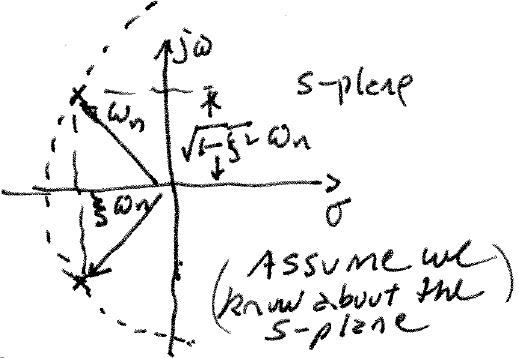
\includegraphics[scale=0.5]{chapter1_s-plane-rep.png}
  \caption{S-Plane representation.}
\end{figure}


\subsection{Passive Network}\index{Filters!Passive Network}

\begin{figure}[h]
  \centering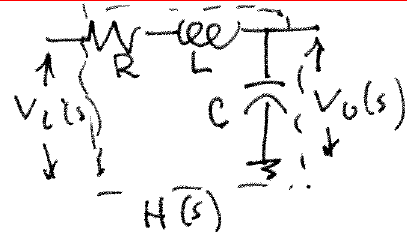
\includegraphics[scale=0.5]{chapter1_passive_filter_network.png}
  \caption{Passive filter network.}
\end{figure}

$$(R+sL)^{-1}(V_i-v_o)=SCv_o $$
$$H(s)=\frac{v_o}{v_i}(s)=\frac{w_n^2}{s^2+2\zeta w_ns+w_n^2} $$
$$w_n=\frac{1}{\sqrt{LC}} \text{ and } \zeta=\frac{R}{2}\sqrt\frac{C}{L}$$

Notice, this approach would most likely need high values of resistance or capacitance and an inductor. High values of R and C are not possible in IC's because they require too much area. In addition, inductors are extremely difficult to fabricate, especially with high Q values.

\subsection{Active Filters}\index{Filters!Active Filters}

\begin{figure}[h]
  \centering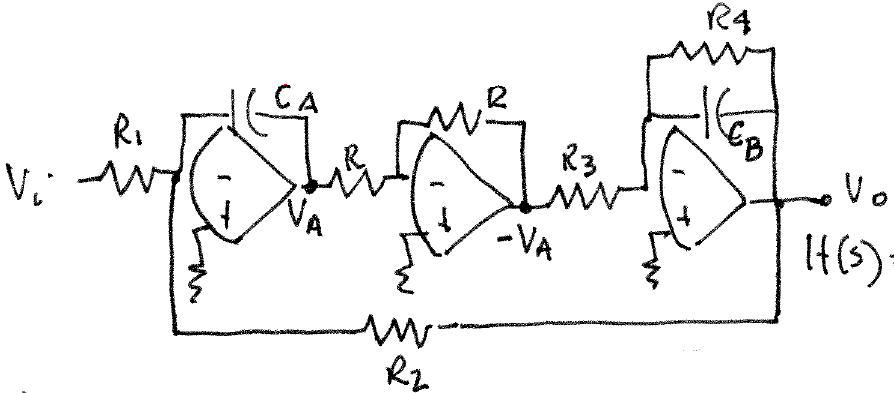
\includegraphics[scale=0.5]{chapter1_active_filter_network.png}
  \caption{Active filter.}
\end{figure}

$$v_Asc_A+R^{-1}v_i+R_2^{-1}v_0=0$$
$$-v_AR_3^{-1}+(R_4^{-1}+sc_B)v_0=0$$
$$H(s)={v_0\over v_i}(s)={-{R_2\over R_1}w_n^2\over s^2+2\zeta w_ns+w_n^2}$$
$$w_n={1\over sqrt{R_2R_3c_Ac_B}} \text{ and } 2\zeta w_n={1\over R_4c_B}$$

\textit{Note: we analyse by summing the currents at the input nodes of the OP AMPS.} \\

If we select R$_1$=R$_2$, then

$$H(s)={-w_n^2\over s^2+s\zeta w_ns+w_n^2}$$

So we can avoid the inductor; however, this would be difficult to integrate on a chip because of the space requirements to realize the RC time constants. For example, let us consider a capacitor of 1 pF with an actual thickness of 700A. We need 3 mil $^2$  to realize this capacitor $(C={k_0\epsilon_0\over t_{ox}}A)$ and capacitors are seldom made larger than 100 pF due to area constraints. Since the LPF needs RC ~ 10$^{-4}$s, for C = 10 pF. $(R=\rho_s({L\over W})$ We need R = 10$^7$ $\Omega$. If we used physical resistors (10$^3$ $\Omega$/square), then we would require 10 $^4$ squares and if the resistor had a width (w) of 10 $\mu$m, then we would need 10$^5\mu m ^2$ ~ 300 mil $^2$. Such large areas are prohibitively large.

\subsection{Switched Capacitor Filter (Sampled Data Filter)}\index{Filters!Switched Capacitor}\index{Filters!Sampled Data}

We can replace the continous time active filter with a discrete-time version by using a switched capacitor to replace the resistor.\\

\begin{figure}[h]
  \centering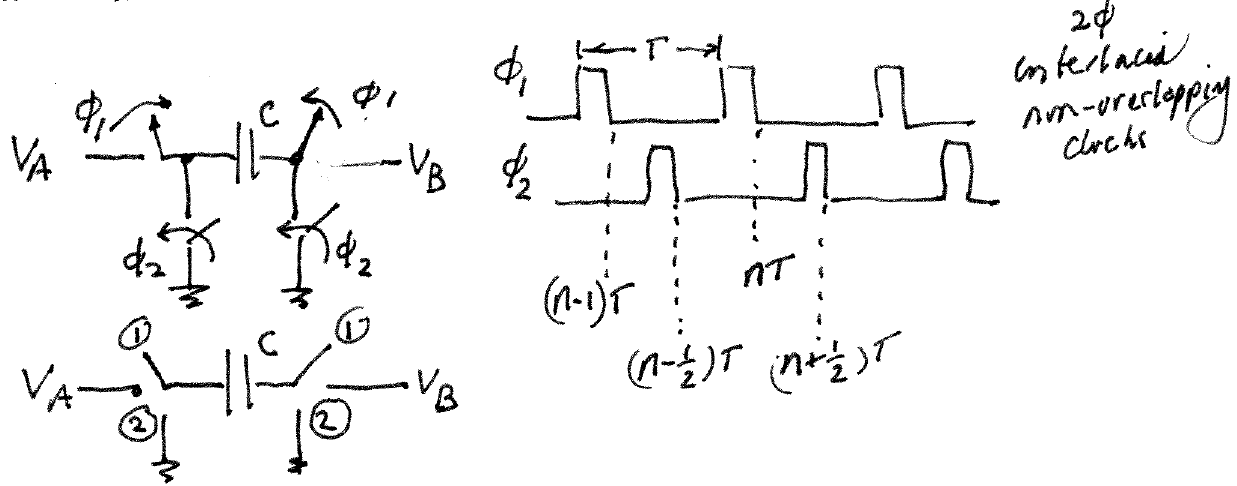
\includegraphics[scale=0.5]{chapter1_switched_capacitor_filter.png}
  \caption{Switched capacitor filter.}
\end{figure}

\begin{multicols}{2}
  \centering $i_{ave}={Q\over T}={C(v_A-v_B)\over T}\triangleq {v_A-v_B\over R}$ \\ $R\triangleq \sfrac{T}{C}={1\over fC}$ \columnbreak \\
  \raggedright With $\phi_2$ closed the capacitor C is discharged to ground, which provides loss for a lossless element. (switched resistor)
\end{multicols}

Now, we consider RC~10$^{-4}$s and set C = 1 pF with f = 1 MHz. We have MATH in area of 3 mil $^2$ which is a reduction if area of 100X. Our new sampled data processor will consist of capacitors, switches and Operational Amplifiers (Op Amps). The clock period (frequency) will be stable and the RC time constants become

$$R_1C_1=T({C_2\over C_1})$$

T is stable, the absolute error is 5-10\% but the ratio error is 0.1-0.5\%

The capacitance ratios have good stability and depend on upon

$$\text{Voltage coefficient } V_V\triangleq{\sfrac{\Delta C}{C}\over \Delta V } \simeq {1\over C}{\partial C\over \partial V} \text{(linearity)}$$
$$\text{Temperature coefficient } V_T\triangleq{\sfrac{\Delta C}{C}\over \Delta T } \simeq {1\over C}{\partial C\over \partial T} \text{(stability)}$$

Thus, our new circuit becomes

\begin{figure}[h]
  \centering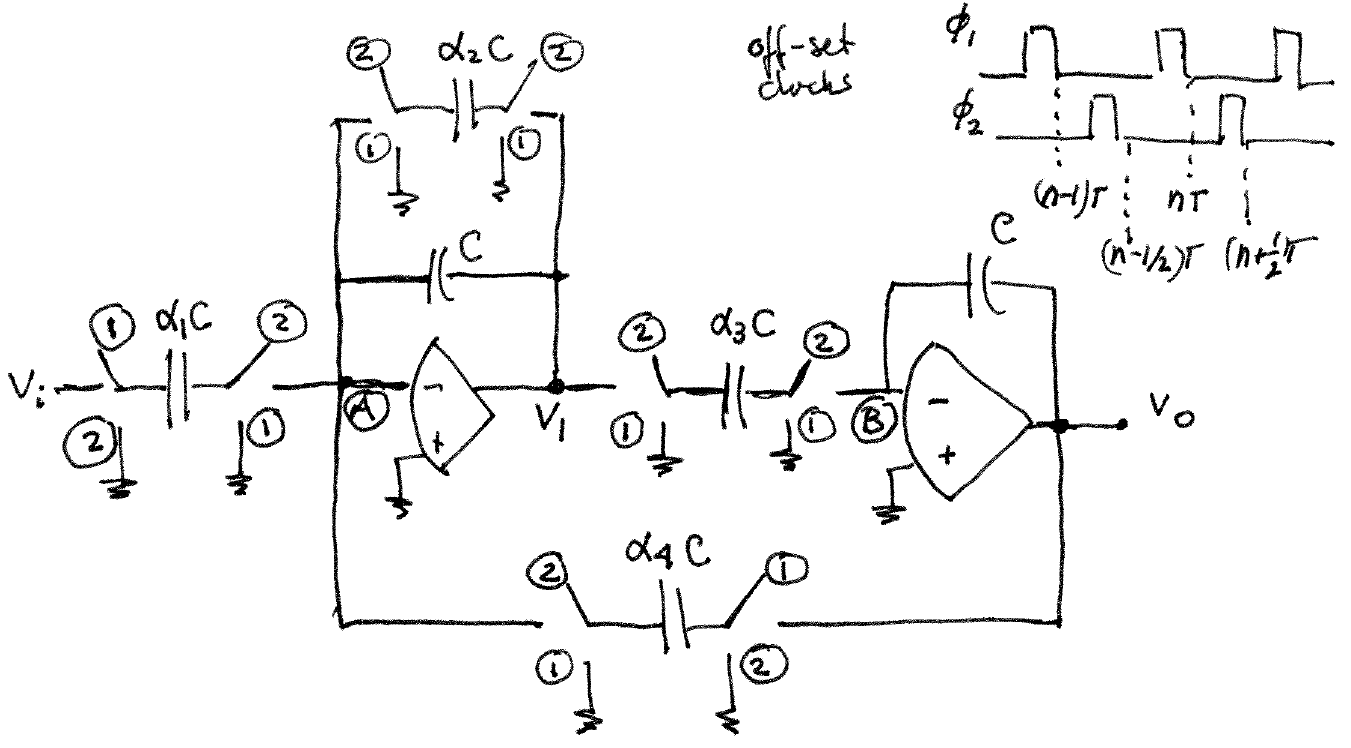
\includegraphics[scale=0.4]{chapter1_active_filter_with_switched_capacitors.png}
  \caption{Active filter implemented with switched capacitors.}
\end{figure}

In the case of continous analog processing (active filters), we summed the currents at the input inverting nodes of the operational amplifiers. For the case of discrete analog signal processing we sum the charges on the capacitors, over a clock cycle, at the summing nodes of the op amps. (This is charge conservation)

\begin{equation}
C[V_1(n)-V_1(n-1)]+\alpha_2 C[V_1(n)-0]+\alpha_1 C[0-V_i(n-1)]+\alpha_4 C[0-V_0(n-1)]=0 \tag{A}
\end{equation}
\begin{equation}
C[V_0(n)-V_0(n-1)]+\alpha_3 C[V_1(n)-0]=0 \tag{B}
\end{equation}


\begin{wrapfigure}{r}{0.2\textwidth}
  \begin{center}
    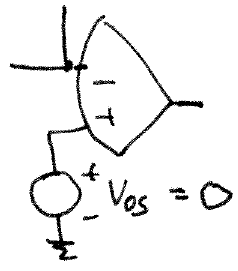
\includegraphics[width=0.2\textwidth]{chapter1_op_amp_with_0_offset.png}
  \end{center}
  \caption{A better model of an Op Amp with a zero offset voltage.}
\end{wrapfigure}

note: we have neglected the off-set voltage of the Op Amps in this analysis and considered the input terminal to be at ground.

We will assume you know something about the so-called Z-transform, where a delay is represented by Z$^{-1} (Z\triangleq e^{sT}$ so we transform the above discrete time equations to the so-called Z-plane.

\begin{equation}
\substack{V_1(z)-Z^{-1}V_1(z)+\alpha_2 v_1(z)-\alpha_1 v_i(z)Z^{-1}-\alpha_4 Z^{-1}V_0(z)=0\\
V_1(z)[1+\alpha_2-Z^{-1}]-\alpha_4V_0(z)Z^{-1}-\alpha_1Z^{-1}V_i(z)=0} \tag{A}
\end{equation}
\begin{equation}
\substack{V_0(z)-V_0(Z)Z^{-1}+\alpha_3V_1(z)=0\\
V_0(z)[1-Z^{-1}]+\alpha_3V_1(z)=0}\tag{B}
\end{equation}

Combining the equations we have

$$H(z)={V_0(z)\over V_i(z)}=\frac{{-\alpha_1\alpha_3\over 1+\alpha_2} Z}{Z^2-[\frac{2+\alpha_2-\alpha_3\alpha_4}{1+\alpha_2}]Z+{1\over 1+\alpha_2}}$$

\begin{wrapfigure}{r}{0.3\textwidth}
  \begin{center}
    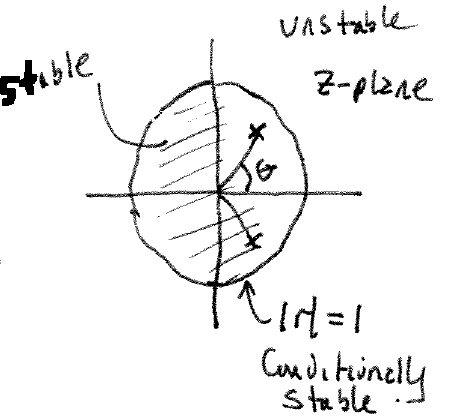
\includegraphics[width=0.3\textwidth]{chapter1_stability_in_z_plane.png}
  \end{center}
  \caption{Stability conditions in the z-plane.}
\end{wrapfigure}

Where the denominator is of the form

$$(z-re^{-i\theta})(z-re^{j\theta})=Z^2-2rcos\theta+r^2$$

So we have $r^2={1\over 1+\alpha_2}\leq1\quad 2rcos\theta={2+\alpha_2-\alpha_3\alpha_4\over 1+\alpha_2}$

We have a pair of complex poles and to find the frequency response we substitute $Z=e^{jwT}=e^{j2\pi(\sfrac{f_s}{f_c})}$ into the transfer function noting that $\\sfrac{f_s}{f_c}\leq\sfrac{1}{2}$ by the Nyquist Criteria. f$_s$= signal frequency and f$_c$ = $\frac{1}{T}$ = clock frequency.

FIGURE

%------------------------------------------------

\section{Sampled Data System}\index{Sampled Data System}

FIGURE

[Problem 1

Given the tranfer function

FIGURE

Show the percent overshoot response to a unit step input $V_i(s)={1\over s}$ is $100 e^{\sfrac{\pi}{\tan\theta}}$ where $\theta$ is the angle determined by the poles with the real axis. If $\theta$ = 45$^o$ ($\zeta=\frac{1}{\sqrt{2}}$) calculate the percent overshoot. This transfer function is a 2-pole, maximally flat magnitude (MFM) Butterworth filter.]

\subsection{Discrete Analog Signal Processing (DASP)}\index{Sampled Data System!Discrete Analog Signal Processing}
\index{Sampled Data System!DASP}

We discuss the basic theory of sampling with a unit sampling function

$$U(T,\tau)$$

FLOATING FIGURE

With period T and pulse duration $\tau$. We apply this sampling function as follows:

FIGURE

We begin by expanding U(T,$\tau$) in a Fourier Series

$$U(\tau,t)=\sum_{n=-\infty}^\infty c_ne^{jnw_st}\quad w_s=2\pi f_s \quad f_s={1\over T}$$

$$\text{With } c_n={1\over T}\int_0^T dt  U(\tau,t)e^{-jnw_st}\left\{
  \begin{array}{l l}
    U(\tau,t) = 1 for kT < t < (k+1)T & \\
    U(\tau,t) = 0 \text{ otherwise} &
  \end{array}\right.$$

[Problem 2

Show by analysis

$$U(\tau,t) = {\tau\over t} + {2\tau\over T}\sum_{n=1}^\infty{\sin({n\pi\tau\over T})\over({n\pi\tau\over T})}\cdot\cos[n(w_st-\phi)]$$

where $\omega_s=2\pi f_s=\frac{2\pi}{T}$ is the fundamental frequency of the pulse train.

$n\phi=n\omega_s(\frac{\tau}{2})$ phase angle of the n$^{th}$ harmonic

$\frac{2\tau}{T}\frac{\sin(n\pi\frac{\tau}{T})}{n\pi\frac{\tau}{T}}$ amplitude of the n$^{th}$ harmonic]

Now, we have

$$f^*(t)=U(\tau,t) f(t)={\tau\over T}f(t) + {2\tau\over T}\sum_{n=1}^\infty{\sin({n\pi\tau\over T})\over ({n\pi\tau\over T})}\cos[n(w_st-\phi)]\cdot f(t)$$

and the frequency spectra is obtained as

$$f(t)=\bigtriangledown\cos(w_0t+\theta_0)={V\over 2}[e^{j(w_0t+\theta_0)}+e^{-j(w_0t+\theta_0)}]$$

which gives

$$f^*(t)={V\tau\over 2T}[e^{j\theta_0}\sum_{n=-\infty}^\infty{\sin({n\pi\tau\over T})\over({n\pi\tau\over T})}e^{-jn\phi}\cdot e^{j(w_0+nw_s)t}+e^{-j\theta_0}\sum_{n=-\infty}^\infty{\sin({n\pi\tau\over T})\over({n\pi\tau\over T})}e^{jn\phi}\cdot e^{-j(w_0+nw_s)t}]$$

with a little manipulation of the indices, with the coefficients of $e^{\pm j(w_0+nw_s)t}$ given as

$$c_n={\tau\over 2T}V{\sin({n\pi\tau\over T})\over ({n\pi\tau\over T})} e^{\pm j(\theta_0-n\phi}=|c_n|e^{\pm j\alpha_n}\text{ and } \alpha_n\triangleq\theta_0-n\phi$$

which illustrates the following:

\begin{itemize}
 \item an infinite number of side lobes (frequencies) $w_0\pm nw_s$
 \item side lobes attenuated by $\frac{\tau}{T}\frac{\sin(n\pi\frac{\tau}{T})}{n\pi\frac{\tau}{T}}$ with
 \item phase components $n\phi=n\omega_s(\frac{\tau}{2}=\frac{n\pi\tau}{T})$
\end{itemize}

Thus, we have the line spectrum for a signal containing one frequency component

FIGURE

When the input signal is a composite periodic wave with 'm' frequency components ranging from 0 to w$_0$ radians/sec, then the frequency spectrum would contain 'm' vertical lines.

FIGURE

We can see if the sampling frequency is such that w$_s$-w$_0$=w$_0$ then there is the possibility of 'overlap' of the frequency spectra, which is called 'aliasing'. In order to prevent this situation we require $w_s\geq 2w_0$, which is called the Nyquist criteria. Under these circumstances, we can pass the output signal through an ideal LPF to recover the input signal. For the case of the single frequency component we have

$$\frac{\tau V}{T}=\cos(\omega_0t+\theta_0)$$

Which is practically the same as the input signal except for the attenuation factor tau/T and the original signal could be recovered through amplification. Thus, sampling leads to the generation of so-called sidebands or 'complementary' signals in a sampled data system, which are undesirable as they bring about 'ripples' or instabilities in a system.

\subsection{Clamping}\index{Sampled Data System!Clamping}

One method of removing the effect of these sidebands on the system is to use a clamping device following the sampling device - a so-called sample/Hold circuit.

FIGURE

The clamping device holds the measured values of the input signal at the sampling instants 0, T, 2T, ... constant for a fraction of the entire sampling period.

FIGURE

If the sampling frequency is greater than twice the signal frequency w$_0$ (assuming a single frequency input) and we pass the clamped signal through a LPF, then the output of the filter is

$$aV{\sin(w_0T_c/2)\over (w_0T_0/2)}\cos(w_0(t-\sfrac{T_c}{2})+\theta_0)$$

which is delayed by half the clamping period and distorted by

$$a{\sin(w_0T_c/2)\over (w_0T_c/2)}$$

Extending this to full-clamping we have an output signal

$$V{\sin(w_0T/2)\over (w_0T/2)}cos(w_0(t-T/2)+\theta_0)$$

FIGURE

The effects of clamping can be studdied in a simple manner by treating the clamping device as a linear network. We treat the input to the clamping device as a train of pulses

$$f^*(t)\to F^*(s)=\sum_{k=0}^Nf_k e^{-kTs}$$

FLOATING FIGURE

$$F_c(s)={1-e^{-T_cS}\over s}\cdot F^*(s)={(1-e^{-T_s})\over s}\sum_{k=0}^Nf_k e^{-kT_s}$$

where f$_k$ is the strength of the k$^{th}$ impulse.

Thus, the transfer function of the clamping device is

$$G_n(s)={1-e^{-T_cs}\over s}$$

and substitution of S=j$\omega$ yields the frequency response,

$$G_n(jw)={1-e^{-jT_cw}\over jw}=2{\sin(wT_c/2)\over w e^{jwT_c/2}}={T_c\over ({wT_c\over 2})}sin({2T_c\over 2})e^{-jwT_c/2}$$

with phase $\phi(w)=-wT_c/2$ of a time delay of half the clamping period.

\subsection{Fundamental Theorem of Sampling}\index{Sampled Data System!Fundamental Theorem of Sampling}
\index{Sampled Data System!Nyquist-Shannon Sampling Theorem}

\textit{Statement}
If F(w), the Fourier Transform of f(t), is band limited

$$F(w)=0 \qquad |w|\geq w_0$$

FIGURE

then f(t) is uniquely determined by its valus at uniform time intervals tha are ${1\over 2f_0}$ seconds apart, namely,

$$f_n(t)\triangleq f({n\over 2f_0})=f({n\pi\over w_0})={1\over 2\pi}\int_{-w_0}^{w_0}\partial wF(w)e^{jw({n\pi\over w_0})}$$

where ${1\over 2\pi}$ is the Nyquist interval and 2f$_0$ the Nyquist frequency.

\textit{Proof}

$$f(t)={1\over 2\pi}\int_{-\infty}^\infty\partial wF(w)e^{jwt}$$
$$t=nT={n\pi\over w_0}\qquad f_n(t){1\over 2\pi}\int_{-\infty}^\infty\partial wF(w)e^{n\pi\over w_0}$$

Sincle F(w) is band limited we can expand in a Fourier series with periodic function $F_p$

$$F_p(w)=\sum_n={-\infty}^\infty c_ne^{-jw(\sfrac{n\pi}{w_0})}\qquad -w_0\leq w\leq w_0$$
$$c_n={1\over 2w_0}\int_{-w_0}^{w_0}\partial wF(w)e^{jw(\sfrac{n\pi}{w_0})}$$

note $F_1(w)=F(w)$ in this frequency interval

FLOATING FIGURE

$$c_n{\pi\over w_0}f_n(t)=Tf(nT)$$

Thus, F(w) is completely described since c$_n$ is known from time samples taken $\frac{1}{2f_0}$ seconds apart to give f$_n$(t). It follows, since F(w) is known, we have f(t).

FLOATING FIGURE

\textit{Reconstruction of f(t)}

$$F_{REC}(w)=P(w)F_P(w)$$
$$\text{ideal filter }=\sum_{-\infty}^\infty c_ne^{-jw{n\pi\over w_0})}=\sum_{-infty}^\infty \underbrace{\pi f_n\over w_0}_{c_n} e^{-jw({n\pi\over w_0})}$$
$$f_{rec}(t)={1\over 2\pi}\int_{-\infty}^\infty\partial wF_{REC}(w)e^{jwt}={\pi\over w_0}\sum_{-\infty}^\infty f_n\int_{-w_o}^{w_0}\partial w e^{jw(t-{n\pi\over w_0})}$$
$$=\sum_{-\infty}^{\infty}f_n(nT) \underbrace{\sin(w_0t-n\pi)\over w_0t-n\pi}_{\mathclap{h_n(t)\text{: impulse response of LPF}}}=\sum_{-\infty}^\infty f_n(n\tau)h_n$$

the function $\frac{\sin\omega_0(t-n\tau)}{\omega_0(t-n\tau)}$ is unity at the n$^{th}$ sampling instant t = nT and zero at all other sampling instants.

FIGURE

In practice we do not select the sampling frequency w$_s$ = $\frac{2\pi}{T}$, but we band limit the input to this system with an anti aliasing filter (AAF).

\subsection{Impulse Sampling S, H, and Z-Transform}\index{Sampled Data System!Impulse Sampling}

FIGURE

For the n$^{th}$ pulse

$$f_n(t)=kf(nT)[U(t-nT)-U(t-nT-\tau)]$$
$$f^*(t)=\sum_{n=0}^\infty f_n(t)=k\sum_{n=0}^\infty f(nT)[U(t-nT)-U(t-nT-\tau)]$$
$$\text{note: }\quad f(t-a)U(t-a)\to e^{-as}F(s)$$
$$U(t)\to \sfrac{1}{s}\quad U(t-\tau)\to {e^{-\tau s}\over s}$$
$$F^*(s)=k\sum_{n=0}^\infty f(nT)[{1\over s} e^{-snT}-{1\over s}e^{-s(nT+\tau)}]$$
$$=k\underbrace{(1-e^{-s\tau})\over s}_{\mathclap{\text{tranform function\\of clamp device}}}\sum_{n=0}^\infty f(nT)e^{-snT}$$

Translation Theorem:\\
$F(s)=\int_0^\infty dtf(t)e^{-st}$\\
$\int_0^\infty dtf(t-a)U(t-a)e^{-st}$\\
let t'=t-a\\
$\int_{-a}^\infty dt'f(t')U(t')e^{-s(t'+a)}$\\
$=\int_0^\infty dtf(t)e^{-st}\cdot e^{-as}$\\
$=e^{-as}F(s)$\\

\textit{Case 1}

We let $\tau\to 0$ and $k\to{1\over \tau}$ (Impulse Sampling)

$$F^*(s)=\sum_{n=0}^\infty f(nT)e^{-snT}$$

Which is the summation of the delayed values of the input signal

$$f(nT)=f(t)\sum_{n=-\infty}^\infty\delta(t-nT)=f(t)\delta_T(t)$$

where $\quad\delta_T(t)=\sum_{-\infty}^\infty\delta(t-nT)$

FLOATING FIGURE

If we let $Z\triangleq e^{sT}$ then

FIGURE

\textit{Case 2}

We let $\tau\to T$ (remove s$_2$ and set k = 1 which means the signal is unchanged between samples (i.e. sample and hold)

$$F^*(s)=\underbrace{(1-e^{-sT})\over s}_\text{transfer function\\ of zero-order\\ sample/Hold circuit}\underbrace{\sum_{n=0}^\infty f(nT)e^{-snT}}_{F_{\sfrac{S}{H}}^*(s)}={(1-e^{-sT})\over s}F^*(s)$$
$$\delta\{F_{\sfrac{S}{H}}(z)\}=F_{\sfrac{S}{H}}(z)=\zeta\{{1-e^{-sT}\over s}\}\zeta\{F^*(s)\}=\zeta\{1-e^{-sT}\}\zeta\{{F^*(s)\over s}\}$$
$$=(1-z^{-1})\zeta\{{F^*()\over s}\}$$

FLOATING FIGURE

The use of Z transforms assumes a sampler at the front and back end of the system.

FIGURE

\subsection{Transformation Between S and Z-planes}\index{Sampled Data System!Transformation Between S and Z-planes}

FIGURE

\subsection{Transfer Functions}\index{Sampled Data System!Transfer Functions}

FIGURE

We will show $G(z)=F(z)\cdot H(z)$

$$G(t)=\sum_{n=0}^\infty g(nT)Z^{-n}\qquad g(t)=\sum_{k=0}^\infty f(kT)h(t-kT)$$
$$g(nt)=\sum_{k=0}^\infty f(kT)h(n-k)T\qquad \text{discrete convolution}$$
$$=\sum_{k=0}^\infty f_kh_{n-k}$$

Let m=n-k

$$G(z)=\sum_{k=0}^\infty \sum_{n=0}^\infty f(kT)h(n-k)TZ^{-n}$$
$$=\sum_{k=0}^\infty \sum_{m=0}^\infty f(kT)h(mT)Z^{-m}\cdot Z^{-k}$$
$$=\sum_{m=0}^\infty h(mT)Z^{-m}\sum_{k=0}^\infty f(kT)Z^{-k}$$
$$=H(z)\cdot F(z)$$

\subsection{Z-Transforms of Simple Functions}\index{Sampled Data System!Z-Transforms of Simple Functions}

\textit{Example 1: Impulse function}

FLOATING FIGURE

$$f(t)=K\delta (t)$$
$$F(s)=\mathcal{L}\{f(t)\}=K\qquad f(nT)=\int_{-\infty}^\infty K\delta(t)dt=\left\{
\begin{array}{l l}
    K & \quad \text{n=0}\\
    0 & \quad \text{otherwise}
  \end{array} \right.$$
  $$F(z)=\sum_{n=0}^\infty f(nT)\underbrace{e^{-snT}}_{Z^{-n}}=K=F(s)$$

Thus, the $\zeta$-transform of an impulse function is the same as the Laplace transform since an impulse function is a pulse function itself!

\textit{Example 2: Step function}

FLOATING FIGURE

$$f(t)=kU(t)$$
$$F(s)=\mathcal{L}\{f(t)\}={K\over s}$$
$$F(t)=\sum_{n=0}^\infty f(nT)Z^{-n}$$
$$=\sum_{n=0}^\infty KZ^{-n}=K[1+Z^{-1}+Z^{-22}+\dots={K\over 1-z^{-1}}|Z^{-1}|<1$$
$$={KZ\over z-1}={K\over 1-Z^{-1}}$$

\textit{Example 3: Ramp function}

FLOATING FIGURE

$$F(s)=\mathcal{L}\{f(t)\}={K\over s^2}$$
$$F(z)=\sum_{n=0}^\infty f(nT)Z^{-n}=\sum_{n=0}^\infty knTZ^{-n}=kTZ^{-1}\left\{1+2Z^{-1}+3Z^{-2}+\dots(k+1)Z^{-k}+\dots\right\}$$
$$={KTZ^{-1}\over(1-Z^{-1})^2}\qquad|Z^{-1}|<1$$
$$={KTZ\over(z-1)^2}$$

\textit{Prob 3: show the following transformations are correct:}

\begin{table}[h]
  \centering
  \begin{tabulary}{1\textwidth}{|l|l|l|}
    \hline
    \textbf{Name} & \textbf{f(t)} & \textbf{F(z)}\\
    \hline
    Delayed Impulse & $K\delta(t-mT)$ & $KZ^{-m}$ \\
    Exponential & $Ke^{-at}$ & ${Ke^{at}Z\over e^{aT}Z-1}={KZ\over Z-e^{-aT}}$ \\
    Sine & $\sin w_0t$ & ${Z\sin w_0T\over Z^2-2\cos w_0TZ+1}$ \\
    Cosine & $\cos w_0t$ & ${Z(Z-\cos w_0 T)\over Z^2-2\cos 2_0TZ+1}$ \\
    \hline
  \end{tabulary}
\end{table}

\subsection{Properties of Z-Transforms and S-Transforms}\index{Sampled Data System!Properties of Z-Transforms and S-Transforms}

\begin{table}[h]
  \centering
  \begin{tabulary}{1\textwidth}{|l|L|L|}
    \hline
    \textbf{Property} & \textbf{Z-Transform} & \textbf{S-Transform}\\
    \hline
    $1^o$ Linearity & $\zeta\{af(t)\}=aF(z)$ & $\substack{\mathcal{L}\{af(t)\}=aF(s)\\
    \mathcal{L}\{f_1(t)\pm f_2(t)\}=F_1(s)\pm F_2(s)}$ \\
    $2^o$ Real transform & $\zeta\{f(t\pm nT)\}=Z^{\pm n} F(z)$ & $\mathcal{L}\{f(t\pm a)\}=e^{\pm as}F(s)$ \\
    $3^o$ Scale change & $\zeta\{e^{\pm at}f(t)\}=F(e^{\mp aT}a)$ & $\substack{\mathcal{L}\{e^{\pm at}f(t)\}=F(s\mp a)\\
    \mathcal{L}\{f(t/a)\}=aF(as)}$ \\
    $4^o$ Convolution & $ \substack{\zeta\{f_1(nt)\otimes f_2(nt)\}\\
    =\sum_{k=0}^\infty f_1(kT)f_2(n-k)T=F_1(z)F_2(z)}$ & $\mathcal{L}\{\int_0^tf_1(\tau)f_2(t-\tau_d\tau\}=F_1(s)\cdot F_2(s)$ \\
    $5^o$ Final value Theorem & $\lim_{z\to 1}\left[(1-z^{-1})F(z)\right]=\lim_{t\to\infty}f(t)$ & $\lim_{s\to 0}[sF(s)]=\lim_{t\to\infty}f(t)$ \\
    $6^o$ Initial value theorem & $\lim_{z\to\infty}[F(s)]=\lim_{t\to 0}f(t)$ & $\lim_{s\to\infty}[sF(s)]=\lim_{t\to 0}f(t)$ \\
    \hline
  \end{tabulary}
\end{table}

%----------------------------------------------------------------------------------------
%	CHAPTER 2
%----------------------------------------------------------------------------------------

\chapterimage{chapter_head_2.pdf} % Chapter heading image

\chapter{Design of Discrete Analog Signal Processors}

\section{Design Strategy for Continuous to Sampled Data Systems}\index{Design Strategies!Continuous to Sampled Data Systems}
\index{Sampled Data System!DASP}

\begin{figure}[h]
  \centering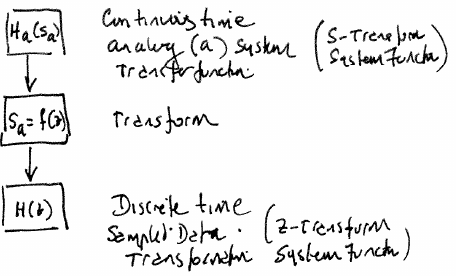
\includegraphics[scale=0.5]{chapter2_figure1.png}
  \caption{I don't really know what this picture is yet. I just put it in.}
\end{figure}

\subsection{Issues to Address in Selection of the Transformations}

T\begin{table}[h]
\centering
\begin{tabulary}{1\textwidth}{L|L|L}
  \underline{Property} & \underline{$H_a(S_a)$} & \underline{$H(z)$} \\
  I. Rational Functions & rational function of $S_a$ selectivity & rational
  function of $z$ selectivity \\
  II. Mapping the Unit Circle for $|x| = 1$ & $s = j\omega_a$ &
  $z=e^{j\omega T}$ (unit circle) \\
  III. Stability $|z|<1$ $Re(S_a) < 0$ & stable (LHP) poles & stable
  poles (inside unit circle) \\
\end{tabulary}
\caption{Selecting the transformation.}
\end{table}

\begin{figure}[h]
  \centering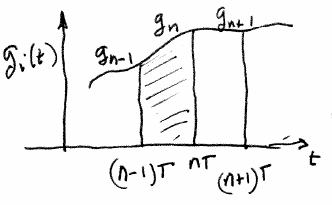
\includegraphics[scale=0.5]{chapter2_figure2.png}
  \caption{I don't really know what this picture is yet. I just put it in.}
\end{figure}

\textit{Approach}
A system funciton $H_a(s_a)$ response can be determined from a collection of $1^{st}$ order differential equations. From the state variable point of view:

$$x_i=\text{ state variable }i = 1, 2, \dots N \text{ state equations }$$
$$g_i = \text{ linear function of }x_i(t) \text{ and the input signal }$$
$${\partial x_i\over \partial t}=g_i(t)$$
$$\text{Laplace transform: }s_ax_i(s_a)=G_i(s_a)\quad i=1,2,3,\dots N\quad x_i(t)=0\quad t<0$$
$$\int_{(n+1)T}^{nT}{\partial x_i\over\partial t} dt=x_i(nT)-x_i[(n-1)T]=\int_{(n-1)T}^{nT}g_i(t)dt$$
We need a $1^{st}$ order difference equation for out sampled data system, which we can develop as
$$X_i(nT)-x_i[(n-1)T]\to(1-z^{-1})X_i(z)$$
but how do we evaluate the $$\zeta$$-transform for $$\int_{(n-1)T}^{nT}g_i(t)dt$$?
Let us examine several approaches:

\subsection{Forward Euler Integrator}

$$\int_{(n-1)T}^{nT}g_i(t)dt\simeq Tg_i[(n-1)T]$$
$$\therefore x_i(nT)-x_i[(n-1)T]=Tg_i[(n-1)T]$$
$$x_i(\tau)-z^{-1}x_i(z)=Tz^{-1}G_i(z)$$
$({z-1\over T})x_i(z)=G_i(z)\Rightarrow$
\begin{tcolorbox}
  ${S_a={z-1\over T}\quad\text{Substitude this expression in transform}}$
\end{tcolorbox}

Let's check out 3 criteria:

\begin{enumerate}
  \item Rational function? OK
  \item Mapping into unit circle? $S_a=\zeta w_a\to Z=1+S_aT=1+jw_aT$\\
  $|z|=1$ only when $w_a=0$ or $w_a\ll\sfrac{1}{T}$ in general not satisfied
  \item Stability? Most complex poles in LHP map into the unit circle, but as the poles approach the jw axis instability may occur.
\end{enumerate}
Zeros do not map from jw axis to the unit circle.

\begin{figure}[h]
  \centering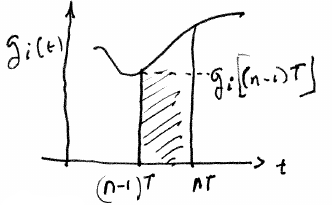
\includegraphics[scale=0.5]{chapter2_figure3.png}
  \caption{I don't really know what this picture is yet. I just put it in.}
\end{figure}

\begin{figure}[h]
  \centering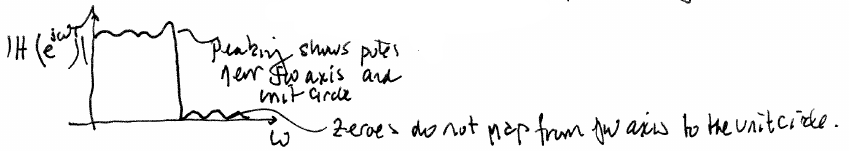
\includegraphics[scale=0.5]{chapter2_figure4.png}
  \caption{I don't really know what this picture is yet. I just put it in.}
\end{figure}

\subsection{Backward Euler Integrator}

\begin{figure}[h]
  \centering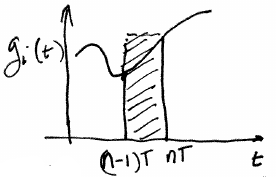
\includegraphics[scale=0.5]{chapter2_figure5.png}
  \caption{I don't really know what this picture is yet. I just put it in.}
\end{figure}

$$\int_{(n-1)T}^{nT}g_i(t)dt\simeq Tg_i(nT)$$
$$x_i(nT)-x_i[(n-1)T]\simeq Tg_i(nT)$$
$$x_i(z)-z^{-1}x_i(t)=TG(z)$$
$$({1-z^{-1}\over T})\cdot X_i(z)=G(z)$$
\begin{tcolorbox}
  let $s_a={1-z^{-1}\over T}={z-1\over ZT}$ do transform
\end{tcolorbox}

\begin{enumerate}
  \item Rational? O.K.
  \item MApping into unit circle? $Z={1\over 1-jw_aT}={1+jw_aT\over 1+w_a^2T^2}$\\
  $|z|=1\text{ only for }w_a=0 (w_a\ll 1/T)$
  \item Stability? Poles move away from unit circle in Z-plane as poles move
  towards $jw_a$ axis in s-plane. Not satisfied.
\end{enumerate}

\subsection{Trapezoidal Integrator (Bilinear Z-Transform)}

$$\int_{(n-1)T}^{nT}g_i(t)dt\simeq{T\over 2}\left[g_i(nT)+g_i[(n-1)T]\right]$$
$$x_i(nT)-x_i[(n-1)T]\simeq{T\over 2}\left[g_i(nT)+g_i[(n-1)T]\right]$$
$$x_i(z)-z^{-1}x_i(z)={T\over 2}[G_i(z)+z^{-1}G_i(z)]$$
$$({2\over T}\underbrace{z-1\over z+1}_{s_a})x_i(z)=G_i(z)\qquad \text{ Select }s_a={2\over T}({z-1\over z+1})$$
\begin{enumerate}
 \item Rational? O.K.
 \item Mapping into unit circle? $s_a=jw_a={2\over T}({z=1\over z+1})$\\
  $jw_{a\over 2}T(z+1)=z-1$\\
  $z(1-jw_{a\over 2}T)=1+jw_{a\over 2}T\quad z={1+jw_{a\over 2}T\over 1-jw_{a\over 2}T} \quad |z|=1 \quad\text{ O.K.}$
  \item Stable? test $s_a=\sigma_a+jw_a\quad\sigma_a<0$
$|z|=\left|{1+\sigma_aT/2+jw_aT/2\over(1-\sigma_{a\over 2}T)-jw_aT/2}\right|<1 \text{ O.K.}$
$jw_a={2\over T}{e^{jwT}-1\over e^{jwT}+1}={2\over T}{e^{jwT\over 2}-e^{-jwT\over 2}\over e^{jwT\over 2}+e^{-jwT\over 2}}=j({2\over T})\tan({wT\over 2})$
$\therefore$
\end{enumerate}
\begin{tcolorbox}
  $${{w_aT\over 2}=\tan({wT\over 2})\text{ or }{wT\over 2}=\tan^{-1}({w_aT\over 2})}$$
\end{tcolorbox}
Which relates the frequency of the continuous time model ($w_a$) to the sampled data frequency (w).
$w\sim w_a\text{ near }w=0,\pm{2\pi\over T}$
Thus, the w-axis (sampled frequency) is warped as compared with the analog frequency $w_a$.

\begin{figure}[h]
  \centering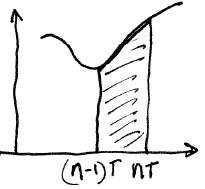
\includegraphics[scale=0.5]{chapter2_figure6.png}
  \caption{I don't really know what this picture is yet. I just put it in.}
\end{figure}

\begin{figure}[h]
  \centering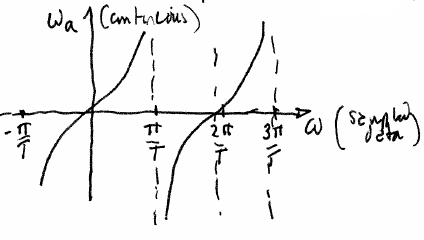
\includegraphics[scale=0.5]{chapter2_figure7.png}
  \caption{I don't really know what this picture is yet. I just put it in.}
\end{figure}

\subsection{Midpoint Integration}

$$\int_{(n-1)T}^{(n+1)T}g_i(t)dt=\int_{(n-1)T}^{(n+1)T}{\partial x_i\over \partial t}=2Tg_i(nT)=x_i[(n+1)T]-x_i[(n-1)T]$$
$$zx_i(z)-z^{-1}x_i(z)=2TG_i(z)$$
$$({z-z^{-1}\over 2T})\cdot x_i(z)=G_i(z)$$
\begin{tcolorbox}
  LDI Transform\\
  $S_a={z-z^{-1}\over 2T}$
\end{tcolorbox}
\begin{enumerate}
 \item Rational? O.K.
 \item Mapping into unit circle? $s_a=jw_a={e^{jwT}-e^{-jwT}\over 2T}={j\sin wT\over T}$\\
 $|z|=|e^{j\sin^{-1}w_aT}|=1\quad w_a={1\over T}\sin wT\to w={1\over T}\sin^{-1}w_aT$\\
 $\therefore\text{ Unit circle of Z-plane maps into }jw_a\text{ axis }$\\
 \item $z_{12}=s_aT\pm\sqrt{1+(s_aT)^2}\text{ if }s_a=jw_a\quad|w_a|\leq\sfrac{1}{T}$\\
 $|z_1|=|z_2|=(w_aT)^2+[1-(w_aT)^2]=1$\\
 and both values lie on the unit circle.\\
 $z_az_2=[s_aT+\sqrt{1+(s_aT)^2}][s_aT-sqrt{1+(s_aT)^2}]=-1$\\
 $therefore z_2=-{1\over z_1}\text{ if }|z_1|<1\text{ then }|z_2|>1\Rightarrow\text{ unstable }$\\
\end{enumerate}

%TABLE

The only transform that satisfies all 3 criteria is the Bilinear Z Transform.
\begin{tcolorbox}
Prob\#4: Show the 3-point Simpson Integration yields the expression
$$\int_{(n-2)T}^{(n+1)T}g_i(t)dt\simeq{T\over 3}\left[g_i[(n-1)T]+g_i[(n+1)T]\right]$$
and find the transformation $s_a=f(z)$. Discuss the 3 conditions requiring the transformation.
\end{tcolorbox}

\begin{figure}[h]
  \centering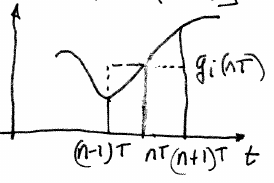
\includegraphics[scale=0.5]{chapter2_figure8.png}
  \caption{I don't really know what this picture is yet. I just put it in.}
\end{figure}

\begin{figure}[h]
  \centering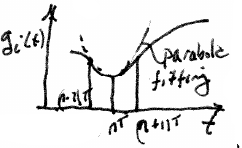
\includegraphics[scale=0.5]{chapter2_figure9.png}
  \caption{I don't really know what this picture is yet. I just put it in.}
\end{figure}

\section{Matching $H(\omega)$ and $H_a(\omega_a)$}

The following conditions are imposed:
\begin{enumerate}
 \item Real part of the denominator must be equal $\Re\{\text{den}H(w)\}=0\text{ at }w_0$
 \item Imaginary part of both denominators must be equal to each other\\
 $\Im{\text{den}H(w)}=\Im{\text{den}H_a(w_a)}|_{w_0}$
 \item Absolute values must be equal at $w_0\quad|H(w_0)|=|H_a(w_0)|
 \item $H(0)=H_a(0)$ D.C. gains must be equal
\end{enumerate}

\begin{figure}[h]
  \centering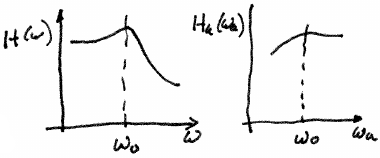
\includegraphics[scale=0.5]{chapter2_figure10.png}
  \caption{I don't really know what this picture is yet. I just put it in.}
\end{figure}

\subsection{Example: Biquad Realization}

\begin{figure}[h]
  \centering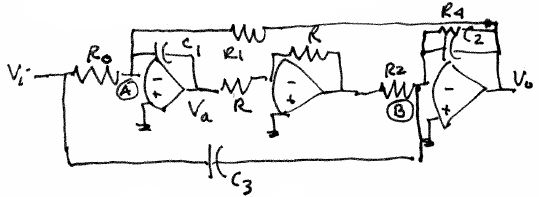
\includegraphics[scale=0.5]{chapter2_figure11.png}
  \caption{I don't really know what this picture is yet. I just put it in.}
\end{figure}

State variable representation of a 2$^{nd}$ order notch function


\begin{figure}[h]
  \centering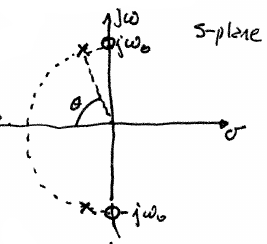
\includegraphics[scale=0.5]{chapter2_figure12.png}
  \caption{I don't really know what this picture is yet. I just put it in.}
\end{figure}
\begin{figure}[h]
  \centering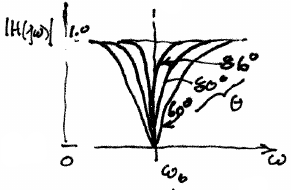
\includegraphics[scale=0.5]{chapter2_figure13.png}
  \caption{I don't really know what this picture is yet. I just put it in.}
\end{figure}
\begin{figure}[h]
  \centering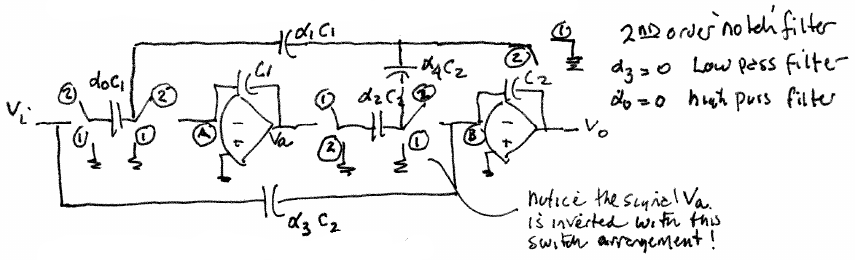
\includegraphics[scale=0.5]{chapter2_figure14.png}
  \caption{I don't really know what this picture is yet. I just put it in.}
\end{figure}
\begin{figure}[h]
  \centering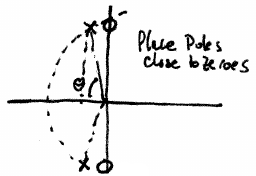
\includegraphics[scale=0.5]{chapter2_figure15.png}
  \caption{I don't really know what this picture is yet. I just put it in.}
\end{figure}
\begin{figure}[h]
  \centering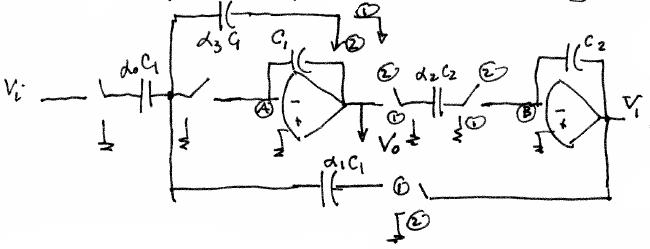
\includegraphics[scale=0.5]{chapter2_figure16.png}
  \caption{I don't really know what this picture is yet. I just put it in.}
\end{figure}

\begin{figure}[h]
  \centering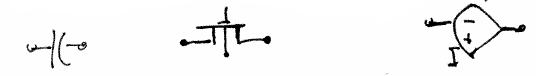
\includegraphics[scale=0.5]{chapter2_figure17.png}
  \caption{I don't really know what this picture is yet. I just put it in.}
\end{figure}

%----------------------------------------------------------------------------------------
%	BIBLIOGRAPHY
%----------------------------------------------------------------------------------------

%\chapter*{Bibliography}
%\addcontentsline{toc}{chapter}{\textcolor{ocre}{Bibliography}}
%\section*{Books}
%\addcontentsline{toc}{section}{Books}
%\printbibliography[heading=bibempty,type=book]
%\section*{Articles}
%\addcontentsline{toc}{section}{Articles}
%\printbibliography[heading=bibempty,type=article]

%----------------------------------------------------------------------------------------
%	INDEX
%----------------------------------------------------------------------------------------

\cleardoublepage
\phantomsection
\setlength{\columnsep}{0.75cm}
\addcontentsline{toc}{chapter}{\textcolor{ocre}{Index}}
\printindex

%----------------------------------------------------------------------------------------

\end{document}
